\documentclass[12pt,letterpaper]{article}
\usepackage[utf8]{inputenc}
\usepackage{listings, float, xcolor}

%----- Configuración del estilo del documento------%
\usepackage{graphicx, fancyhdr, lastpage}
\usepackage{enumitem, pifont, hyperref, ulem}
\usepackage[left=2cm,right=2cm,top=1.8cm,bottom=2.3cm]{geometry}

\pagestyle{fancy}
\fancyhf{}
\rfoot{\textit{Página \thepage \hspace{1pt} de \pageref{LastPage}}}

%------ Paquetes matemáticos básicos --------%
\usepackage{amsmath, amssymb, amsthm}

%------ Definimos los colores para la sintaxis del código --------%
\definecolor{keywordcolor}{rgb}{0.5, 0.0, 0.5} % Morado para palabras clave
\definecolor{commentcolor}{rgb}{0.25, 0.5, 0.35} % Verde para comentarios
\definecolor{stringcolor}{rgb}{0.58, 0.0, 0.82} % Púrpura para strings

%------ Configuración para mostrar código VHDL  --------%
\lstdefinestyle{vhdlstyle}{
    language=VHDL,
    basicstyle=\ttfamily\footnotesize,
    keywordstyle=\color{keywordcolor}\bfseries,
    commentstyle=\color{commentcolor},
    stringstyle=\color{stringcolor},
    numbers=left,
    numberstyle=\tiny,
    stepnumber=1,
    numbersep=5pt,
    backgroundcolor=\color{gray!10},
    tabsize=2,
    showspaces=false,
    showstringspaces=false,
    breaklines=true,
    frame=single,
    captionpos=b
}

%------ Personalizar el link al video  --------%
\hypersetup{
    colorlinks=true,
    linkcolor=blue!50!black, % Azul oscuro
    urlcolor=blue!50!black,  % Azul oscuro
    hidelinks % Elimina el recuadro azul
}

\begin{document}

%------ Encabezado -------- %
\begin{center}
\newcommand{\imp}{\rightarrow}
\newcommand{\vp}{\varphi}
  \begin{minipage}{3cm}
    \begin{center}
      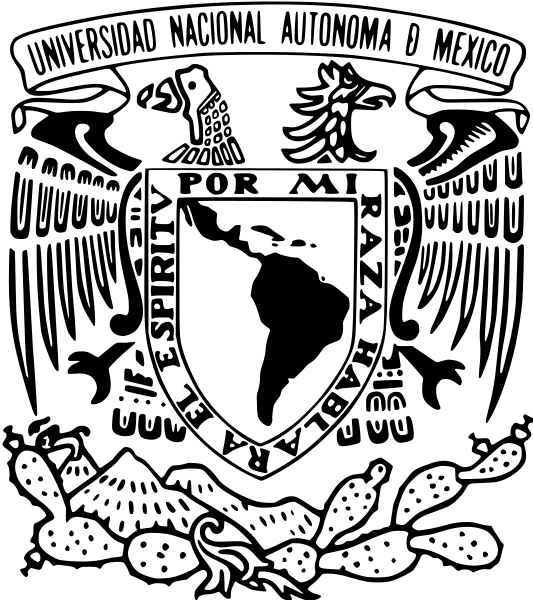
\includegraphics[height=3.4cm]{../unam_logo.png}
    \end{center}
  \end{minipage}\hfill
  \begin{minipage}{10cm}
    \begin{center}
      \textbf{\Large Universidad Nacional Autónoma de México}\\[0.2cm]
      \textbf{\large Facultad de Ciencias}\\[0.2cm]
      \textbf{Organización y Arquitectura de Computadoras 2025-2}\\[0.4cm]
      \textbf{\Large Práctica 04}\\[0.1cm]
      \textbf{Docentes:}\\
      José Galaviz \hspace{1em} Ricardo Pérez \hspace{1em} Ximena Lezama\\[0.3cm]
      \textbf{Autores:}\\
      Fernanda Ramírez Juárez \quad Ianluck Rojo Peña\\[0.3cm]
      \textbf{Fecha de entrega:} Jueves 06 de marzo de 2025
    \end{center}
  \end{minipage}\hfill
  \begin{minipage}{3cm}
    \begin{center}
      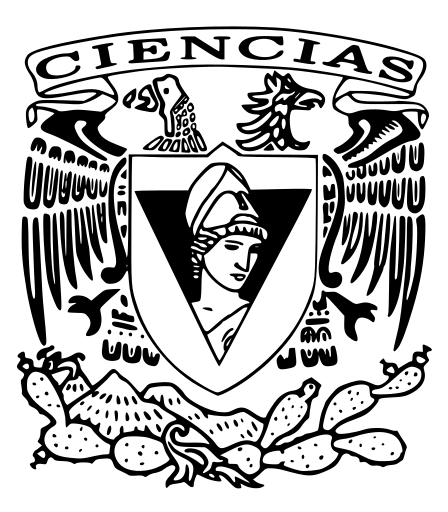
\includegraphics[height=3.4cm]{../fc_logo.png}
    \end{center}
  \end{minipage}
\end{center}

\bigskip
\hrule height 0.1pt
\bigskip

%------ Contenido -------- %
\section*{Preguntas.}

\begin{enumerate}
\item ¿Qu\'{e} es VHDL? ¿C\'{o}mo se ve un full-adder en VHDL? y ¿C\'{o}mo se ve un Half-Adder?
  
    \bigskip
    % -- Respuesta -- %
    \textbf{Aviso.} El contenido de la respuesta a esta pregunta fue obtenida de la siguiente p\'{a}gina:\\
    \href{https://surf-vhdl.com/how-to-implement-a-full-adder-in-vhdl/}{\textit{\uline{How to Implement a Full Adder in VHDL}}}\\
    VHDL \textit{(La V significa \textbf{VHSIC (Very High Speed Integrated Circuits)}, VHSIC Hardware Description Language)} es un lenguaje de descripción de circuitos electrónicos digitales que utiliza distintos niveles de abstracción.
    Permite acelerar el proceso de diseño.
    No es un lenguaje de programación, por ello conocer su sintaxis no implica necesariamente saber diseñar con él, en cambio VHDL es un lenguaje de descripción de hardware, que permite describir circuitos síncronos y asíncronos. En particular permite tanto una descripción de la estructura del circuito, como la especificación de la funcionalidad de un circuito utilizando formas familiares a los lenguajes de programación.
   
    A continuaci\'{o}n se muestra un ejemplo del sumador completo. En el código VHDL, este está implementado en la línea 24 sobre la entrada registrada. N\'{o}tese que, antes de realizar la operación de suma, se extiende el número de bits del operando de entrada. Esto se implementa utilizando la función estándar “resize” proporcionada en el paquete $“numeric_std”$, como se muestra en las líneas 31 y 32.\\

    \begin{lstlisting}[style=vhdlstyle, caption={Código VHDL - Sumador con Registro}]
      library ieee;
      use ieee.std_logic_1164.all;
      use ieee.numeric_std.all;

      entity adder_full_signed_reg is
      generic(
        N             : integer := 8);
      port (
        i_clk       : in     std_logic;
        i_add1      : in     std_logic_vector(N-1 downto 0);
        i_add2      : in     std_logic_vector(N-1 downto 0);
        o_sum       : out    std_logic_vector(N downto 0));
      end adder_full_signed_reg;
        
      architecture rtl of adder_full_signed_reg is
        
      signal r_add1   : signed(N downto 0);
      signal r_add2   : signed(N downto 0);
      signal w_sum    : signed(N downto 0);
      
      begin
      
      -- combinatorial adder
        w_sum <= r_add1 + r_add2;
        
      r_process : process(i_clk)
      begin
        if(rising_edge(i_clk)) then

        -- register input and extend sign
          r_add1      <=  resize(signed(i_add1),N+1);
          r_add2      <=  resize(signed(i_add2),N+1);
        
        -- register output
          o_sum       <= std_logic_vector(w_sum);
        
        end if;
      end process r_process;

      end rtl;
    \end{lstlisting}
    
    En el ejemplo, se implementa un sumador completo con signo. Para un sumador completo sin signo, solo es cuesti\'{o}n de reemplazar la línea que contiene la definición del tipo de datos “signed” por “unsigned”.\\
    
    \begin{lstlisting}[style=vhdlstyle, caption={Código VHDL - Sumador sin Registro}]
      library ieee;
      use ieee.std_logic_1164.all;
      use ieee.numeric_std.all;
      
      entity adder_full_unsigned is
      generic(
        N        : integer := 8);
      port (
        add1     : in     std_logic_vector(N-1 downto 0);
        add2     : in     std_logic_vector(N-1 downto 0);
        sum      : out    std_logic_vector(N downto 0));
      end adder_full_unsigned;
      
      architecture rtl of adder_full_unsigned is
      
      begin
      
        sum <= std_logic_vector( resize(unsigned(add1),N+1) + resize(unsigned(add2),N+1) );

      end rtl;
    \end{lstlisting}
    
    En este caso, el sumador es puramente combinacional.
    VHDL código para Half Adder:\\
    \begin{lstlisting}[style=vhdlstyle, caption={Código VHDL - Medio Sumador}]
      library ieee;
      use ieee.std_logic_1164.all;
      use ieee.numeric_std.all;

      entity adder_half_unsigned_reg is
      generic(
        N       : integer := 256);
      port (
        i_clk     : in     std_logic;
        i_add1    : in     std_logic_vector(N-1 downto 0);
        i_add2    : in     std_logic_vector(N-1 downto 0);
        o_sum     : out    std_logic_vector(N-1 downto 0));
      end adder_half_unsigned_reg;

      architecture rtl of adder_half_unsigned_reg is

      signal r_add1    : unsigned(N-1 downto 0);
      signal r_add2    : unsigned(N-1 downto 0);
      signal w_sum     : unsigned(N-1 downto 0);

      begin

      -- combinatorial adder
        w_sum <= r_add1 + r_add2;

      r_process : process(i_clk)
      begin
        if(rising_edge(i_clk)) then
      
        -- register input
          r_add1      <=  unsigned(i_add1);
          r_add2      <=  unsigned(i_add2);
      
        -- register output
          o_sum       <= std_logic_vector(w_sum);
      
        end if;
      end process r_process;

      end rtl;
    \end{lstlisting}
    \bigskip
  \item En el contexto de las ALUs, explica qu\'{e} son los: SIMD, MIMD, La Execution Units (EUs) y
los Address Generation Units (AGUs).
    
    \bigskip
    % -- Respuesta -- % 
    En el contexto de las ALUs (Unidades Aritmético-Lógicas), se utilizan diversas técnicas y unidades especializadas para aumentar el rendimiento y el paralelismo.
    \begin{itemize}
    \item \textbf{SIMD (Single Instruction, Multiple Data):} Técnica de procesamiento paralelo en la que una sola instrucción se aplica simultáneamente a múltiples datos. Permite que una ALU procese varios elementos de datos en paralelo, aumentando la eficiencia en tareas que involucran operaciones repetitivas. Muy útil en el procesamiento de vectores, imágenes, audio o cualquier tarea donde la misma operación se deba realizar sobre muchos elementos. Es clave en unidades como AVX en CPUs y en GPUs modernas.
    
    \item \textbf{MIMD (Multiple Instruction, Multiple Data):} Arquitectura en la que múltiples procesadores ejecutan diferentes instrucciones sobre distintos datos de manera independiente. Facilita la multitarea y la ejecución concurrente de programas complejos, mejorando el rendimiento en entornos con cargas de trabajo heterogéneas. Es fundamental para la computación paralela, con aplicaciones en simulaciones, modelado y diseño asistido.

    \item \textbf{Execution Units (EUs):} Unidades dentro del procesador responsables de ejecutar instrucciones. Pueden incluir ALUs y otras unidades especializadas en operaciones de punto flotante o enteras. Durante la ejecución de un programa, las EUs reciben las instrucciones decodificadas y realizan los cálculos o las operaciones correspondientes. Permiten la ejecución paralela y especializada de distintas operaciones, lo que optimiza el rendimiento general del procesador mediante técnicas como la ejecución en paralelo y el pipelining.
    
    \item \textbf{Address Generation Units (AGUs):} Unidades dedicadas al cálculo de direcciones de memoria necesarias para las operaciones de carga y almacenamiento, optimizando el acceso a los datos. Cuando se necesita acceder a una posición de memoria, las AGUs calculan la dirección efectiva a partir de una base, un offset y, en ocasiones, una escala. Al separar el cálculo de direcciones de las operaciones aritméticas y lógicas, se agiliza el acceso a la memoria, permitiendo que la CPU opere de manera más eficiente al realizar múltiples tareas en paralelo.
    
    En conjunto, estos elementos permiten mejorar la eficiencia del procesamiento de datos y la ejecución de instrucciones en arquitecturas modernas de computación.
    \end{itemize}
    \bigskip
    
  \item ¿Qu\'{e} es el Carry-Look-Ahead Adder?
    
    \bigskip
    % -- Respuesta -- %
    El \textit{Carry-Look-Ahead Adder \textbf{(Sumador de Acarreo Anticipado, CLA)}} es un tipo de sumador digital diseñado para realizar operaciones aritméticas de forma rápida y eficiente, reduciendo el tiempo de espera asociado a la propagación del acarreo en sumadores tradicionales como el \textit{Ripple Carry Adder}.
    
    \textbf{Características:}
    \begin{itemize}
    \item Se introdujo en 1958 y ha sido la base de varias modificaciones e implementaciones en circuitos digitales.
    \item Calcula uno o más bits de acarreo antes de la suma, evitando la propagación secuencial del acarreo.
    \item Reduce el tiempo de propagación, lo que permite una ejecución más rápida de operaciones aritméticas.
    \item Se utiliza en diseños de procesadores, especialmente en operaciones de multiplicación y división.
    \end{itemize}

    \textbf{Funcionamiento:}
    El CLA emplea dos señales clave para determinar cómo se propagan los acarreos:
    \begin{itemize}
    \item Carry Generate (G): Indica que una posición generará un acarreo independientemente del acarreo de entrada.
    \item Carry Propagate (P): Indica que un acarreo de entrada se propagará a la siguiente posición.
    \end{itemize}
    Para cada posición de bit, el CLA analiza si se generará un acarreo o si se propagará el acarreo desde una posición anterior. Al calcular estos valores en paralelo, el CLA puede deducir rápidamente los acarreos sin esperar a que se propaguen bit por bit.
    
    \textbf{Ventajas:}
    \begin{itemize}
    \item Mayor velocidad. Reduce el retraso de propagación del acarreo, acelerando las sumas de múltiples bits.
    \item Mejor rendimiento en circuitos de gran tamaño. Especialmente útil en ALUs.
    \item Optimización con unidades de acarreo anticipado (LCU). Se utilizan junto con el CLA para calcular acarreos de manera más eficiente en sumadores de mayor tamaño.
    \end{itemize}

    \bigskip
\end{enumerate}

\section*{Punto Extra.}
Link al video para el punto extra:
\href{https://drive.google.com/file/d/1P7wGbd6McrWZda3zwOVueDhKDfkiJzHR/view?usp=drivesdk}{\textit{\uline{Compuertas Lógicas en Minecraft}}}
\end{document}
